
\columnratio{0.55}
\begin{paracol}{2} 
 
\switchcolumn[0]*%%%%%%%
\section{Composition API FAQ}
\switchcolumn
\section{组合式 API 常见问答}
\switchcolumn[0]*%%%%%%%
\begin{vueQuote}{TIP}
This FAQ assumes prior experience with Vue - in particular, experience
with Vue 2 while primarily using Options API.
\end{vueQuote} 
\switchcolumn
\begin{vueQuote}{TIP}
这个 FAQ 假定你已经有一些使用 Vue 的经验,特别是用选项式 API 使用 Vue 2
的经验。
\end{vueQuote} 
\switchcolumn[0]*%%%%%%%
\subsection{What is Composition API?}
\switchcolumn
\subsection{什么是组合式 API?}
\switchcolumn[0]*%%%%%%%
Composition API is a set of APIs that allows us to author Vue components
using imported functions instead of declaring options. It is an umbrella
term that covers the following APIs:
\switchcolumn
组合式 API (Composition API) 是一系列 API
的集合,使我们可以使用函数而不是声明选项的方式书写 Vue
组件。它是一个概括性的术语,涵盖了以下方面的 API:
\switchcolumn[0]*%%%%%%%
\begin{itemize}
\item
  \href{https://vuejs.org/api/reactivity-core.html}{Reactivity API},
  e.g. \texttt{ref()} and \texttt{reactive()}, that allows us to
  directly create reactive state, computed state, and watchers.
\item
  \href{https://vuejs.org/api/composition-api-lifecycle.html}{Lifecycle
  Hooks}, e.g. \texttt{onMounted()} and \texttt{onUnmounted()}, that
  allow us to programmatically hook into the component lifecycle.
\item
  \href{https://vuejs.org/api/composition-api-dependency-injection.html}{Dependency
  Injection}, i.e. \texttt{provide()} and \texttt{inject()}, that allow
  us to leverage Vue's dependency injection system while using
  Reactivity APIs.
\end{itemize}
\switchcolumn
\begin{itemize}
\item
  \href{https://cn.vuejs.org/api/reactivity-core.html}{响应式 API}:例如
  \texttt{ref()} 和
  \texttt{reactive()},使我们可以直接创建响应式状态、计算属性和侦听器。
\item
  \href{https://cn.vuejs.org/api/composition-api-lifecycle.html}{生命周期钩子}:例如
  \texttt{onMounted()} 和
  \texttt{onUnmounted()},使我们可以在组件各个生命周期阶段添加逻辑。
\item
  \href{https://cn.vuejs.org/api/composition-api-dependency-injection.html}{依赖注入}:例如
  \texttt{provide()} 和 \texttt{inject()},使我们可以在使用响应式 API
  时,利用 Vue 的依赖注入系统。
\end{itemize}
\switchcolumn[0]*%%%%%%%
Composition API is a built-in feature of Vue 3 and
\href{https://blog.vuejs.org/posts/vue-2-7-naruto.html}{Vue 2.7}. For
older Vue 2 versions, use the officially maintained
\href{https://github.com/vuejs/composition-api}{\texttt{@vue/composition-api}}
plugin. In Vue 3, it is also primarily used together with the
\href{https://vuejs.org/api/sfc-script-setup.html}{``} syntax in
Single-File Components. Here's a basic example of a component using
Composition API:
\switchcolumn
组合式 API 是 Vue 3 及
\href{https://blog.vuejs.org/posts/vue-2-7-naruto.html}{Vue 2.7}
的内置功能。对于更老的 Vue 2 版本,可以使用官方维护的插件
\href{https://github.com/vuejs/composition-api}{\texttt{@vue/composition-api}}。在
Vue 3 中,组合式 API 基本上都会配合
\href{https://cn.vuejs.org/api/sfc-script-setup.html}{``}
语法在单文件组件中使用。下面是一个使用组合式 API 的组件示例:
\switchcolumn[0]*%%%%%%%
\begin{codeHtml}
<script setup>
import { ref, onMounted } from 'vue'
// 响应式状态
const count = ref(0)
// 更改状态、触发更新的函数
function increment() {
  count.value++
}
// 生命周期钩子
onMounted(() => {
  console.log(`计数器初始值为 ${count.value}。`)
})
</script>
<template>
  <button @click="increment">点击了:{{ count }} 次</button>
</template>
\end{codeHtml}
\switchcolumn
\begin{codeHtml}
<script setup>
import { ref, onMounted } from 'vue'
// 响应式状态
const count = ref(0)
// 更改状态、触发更新的函数
function increment() {
  count.value++
}
// 生命周期钩子
onMounted(() => {
  console.log(`计数器初始值为 ${count.value}。`)
})
</script>
<template>
  <button @click="increment">点击了:{{ count }} 次</button>
</template>
\end{codeHtml}
\switchcolumn[0]*%%%%%%%
Despite an API style based on function composition, \textbf{Composition
API is NOT functional programming}. Composition API is based on Vue's
mutable, fine-grained reactivity paradigm, whereas functional
programming emphasizes immutability.
\switchcolumn
虽然这套 API 的风格是基于函数的组合,但\textbf{组合式 API
并不是函数式编程}。组合式 API 是以 Vue
中数据可变的、细粒度的响应性系统为基础的,而函数式编程通常强调数据不可变。
\switchcolumn[0]*%%%%%%%
If you are interested in learning how to use Vue with Composition API,
you can set the site-wide API preference to Composition API using the
toggle at the top of the left sidebar, and then go through the guide
from the beginning.
\switchcolumn
如果你对如何通过组合式 API 使用 Vue
感兴趣,可以通过页面左侧边栏上方的开关将 API 偏好切换到组合式
API,然后重新从头阅读指引。
\end{paracol}



\columnratio{0.55}
\begin{paracol}{2} 
 
\switchcolumn[0]*%%%%%%%
\subsection{Why Composition API?}
\switchcolumn
\subsection{为什么要有组合式 API?}
\switchcolumn[0]*%%%%%%%
\subsubsection{Better Logic Reuse}
\switchcolumn
\subsubsection{更好的逻辑复用}
\switchcolumn[0]*%%%%%%%
The primary advantage of Composition API is that it enables clean,
efficient logic reuse in the form of
\href{https://vuejs.org/guide/reusability/composables.html}{Composable
functions}. It solves
\href{https://vuejs.org/guide/reusability/composables.html\#vs-mixins}{all
the drawbacks of mixins}, the primary logic reuse mechanism for Options
API.
\switchcolumn
组合式 API
最基本的优势是它使我们能够通过\href{https://cn.vuejs.org/guide/reusability/composables.html}{组合函数}来实现更加简洁高效的逻辑复用。在选项式
API 中我们主要的逻辑复用机制是 mixins,而组合式 API 解决了
\href{https://cn.vuejs.org/guide/reusability/composables.html\#vs-mixins}{mixins
的所有缺陷}。
\switchcolumn[0]*%%%%%%%
Composition API's logic reuse capability has given rise to impressive
community projects such as \href{https://vueuse.org/}{VueUse}, an
ever-growing collection of composable utilities. It also serves as a
clean mechanism for easily integrating stateful third-party services or
libraries into Vue's reactivity system, for example
\href{https://vuejs.org/guide/extras/reactivity-in-depth.html\#immutable-data}{immutable
data},
\href{https://vuejs.org/guide/extras/reactivity-in-depth.html\#state-machines}{state
machines}, and
\href{https://vuejs.org/guide/extras/reactivity-in-depth.html\#rxjs}{RxJS}.
\switchcolumn
组合式 API 提供的逻辑复用能力孵化了一些非常棒的社区项目,比如
\href{https://vueuse.org/}{VueUse},一个不断成长的工具型组合式函数集合。组合式
API 还为其他第三方状态管理库与 Vue
的响应式系统之间的集成提供了一套简洁清晰的机制,例如\href{https://cn.vuejs.org/guide/extras/reactivity-in-depth.html\#immutable-data}{不可变数据}、\href{https://cn.vuejs.org/guide/extras/reactivity-in-depth.html\#state-machines}{状态机}与
\href{https://cn.vuejs.org/guide/extras/reactivity-in-depth.html\#rxjs}{RxJS}。
\switchcolumn[0]*%%%%%%%
\subsubsection{More Flexible Code Organization}
\switchcolumn
\subsubsection{更灵活的代码组织}
\switchcolumn[0]*%%%%%%%
Many users love that we write organized code by default with Options
API: everything has its place based on the option it falls under.
However, Options API poses serious limitations when a single component's
logic grows beyond a certain complexity threshold. This limitation is
particularly prominent in components that need to deal with multiple
\textbf{logical concerns}, which we have witnessed first hand in many
production Vue 2 apps.
\switchcolumn
许多用户喜欢选项式 API
的原因是它在默认情况下就能够让人写出有组织的代码:大部分代码都自然地被放进了对应的选项里。然而,选项式
API
在单个组件的逻辑复杂到一定程度时,会面临一些无法忽视的限制。这些限制主要体现在需要处理多个\textbf{逻辑关注点}的组件中,这是我们在许多
Vue 2 的实际案例中所观察到的。
\switchcolumn[0]*%%%%%%%
Take the folder explorer component from Vue CLI's GUI as an example:
this component is responsible for the following logical concerns:
\switchcolumn
我们以 Vue CLI GUI
中的文件浏览器组件为例:这个组件承担了以下几个逻辑关注点:
\switchcolumn[0]*%%%%%%%
\begin{itemize}
\item
  Tracking current folder state and displaying its content
\item
  Handling folder navigation (opening, closing, refreshing...)
\item
  Handling new folder creation
\item
  Toggling show favorite folders only
\item
  Toggling show hidden folders
\item
  Handling current working directory changes
\end{itemize}
\switchcolumn
\begin{itemize}
\item
  追踪当前文件夹的状态,展示其内容
\item
  处理文件夹的相关操作 (打开、关闭和刷新)
\item
  支持创建新文件夹
\item
  可以切换到只展示收藏的文件夹
\item
  可以开启对隐藏文件夹的展示
\item
  处理当前工作目录中的变更
\end{itemize}
\switchcolumn[0]*%%%%%%%
The
\href{https://github.com/vuejs/vue-cli/blob/a09407dd5b9f18ace7501ddb603b95e31d6d93c0/packages/@vue/cli-ui/src/components/folder/FolderExplorer.vue\#L198-L404}{original
version} of the component was written in Options API. If we give each
line of code a color based on the logical concern it is dealing with,
this is how it looks:
\switchcolumn
这个组件\href{https://github.com/vuejs/vue-cli/blob/a09407dd5b9f18ace7501ddb603b95e31d6d93c0/packages/@vue/cli-ui/src/components/folder/FolderExplorer.vue\#L198-L404}{最原始的版本}是由选项式
API 写成的。如果我们为相同的逻辑关注点标上一种颜色,那将会是这样:
\end{paracol}

\begin{center} 
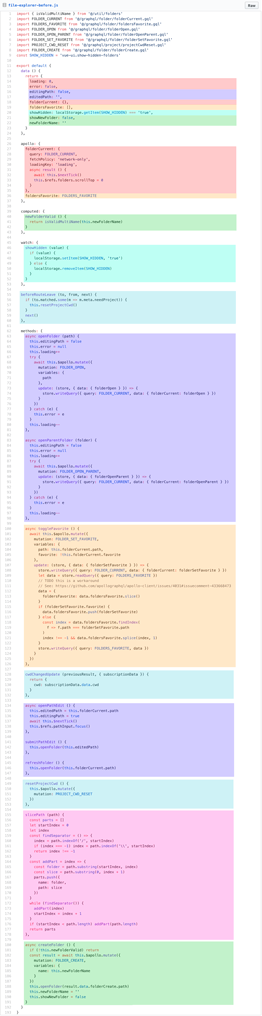
\includegraphics{./img/62783021-7ce24400-ba89-11e9-9dd3-36f4f6b1fae2.png} 
\end{center}
    

\columnratio{0.55}
\begin{paracol}{2} 
 
\switchcolumn[0]*%%%%%%%
Notice how code dealing with the same logical concern is forced to be
split under different options, located in different parts of the file.
In a component that is several hundred lines long, understanding and
navigating a single logical concern requires constantly scrolling up and
down the file, making it much more difficult than it should be. In
addition, if we ever intend to extract a logical concern into a reusable
utility, it takes quite a bit of work to find and extract the right
pieces of code from different parts of the file.
\switchcolumn
你可以看到,处理相同逻辑关注点的代码被强制拆分在了不同的选项中,位于文件的不同部分。在一个几百行的大组件中,要读懂代码中的一个逻辑关注点,需要在文件中反复上下滚动,这并不理想。另外,如果我们想要将一个逻辑关注点抽取重构到一个可复用的工具函数中,需要从文件的多个不同部分找到所需的正确片段。
\switchcolumn[0]*%%%%%%%
Here's the same component, before and after the
\href{https://gist.github.com/yyx990803/8854f8f6a97631576c14b63c8acd8f2e}{refactor
into Composition API}:
\switchcolumn
而如果\href{https://gist.github.com/yyx990803/8854f8f6a97631576c14b63c8acd8f2e}{用组合式
API 重构}这个组件,将会变成下面右边这样:
\end{paracol}

\begin{center} 
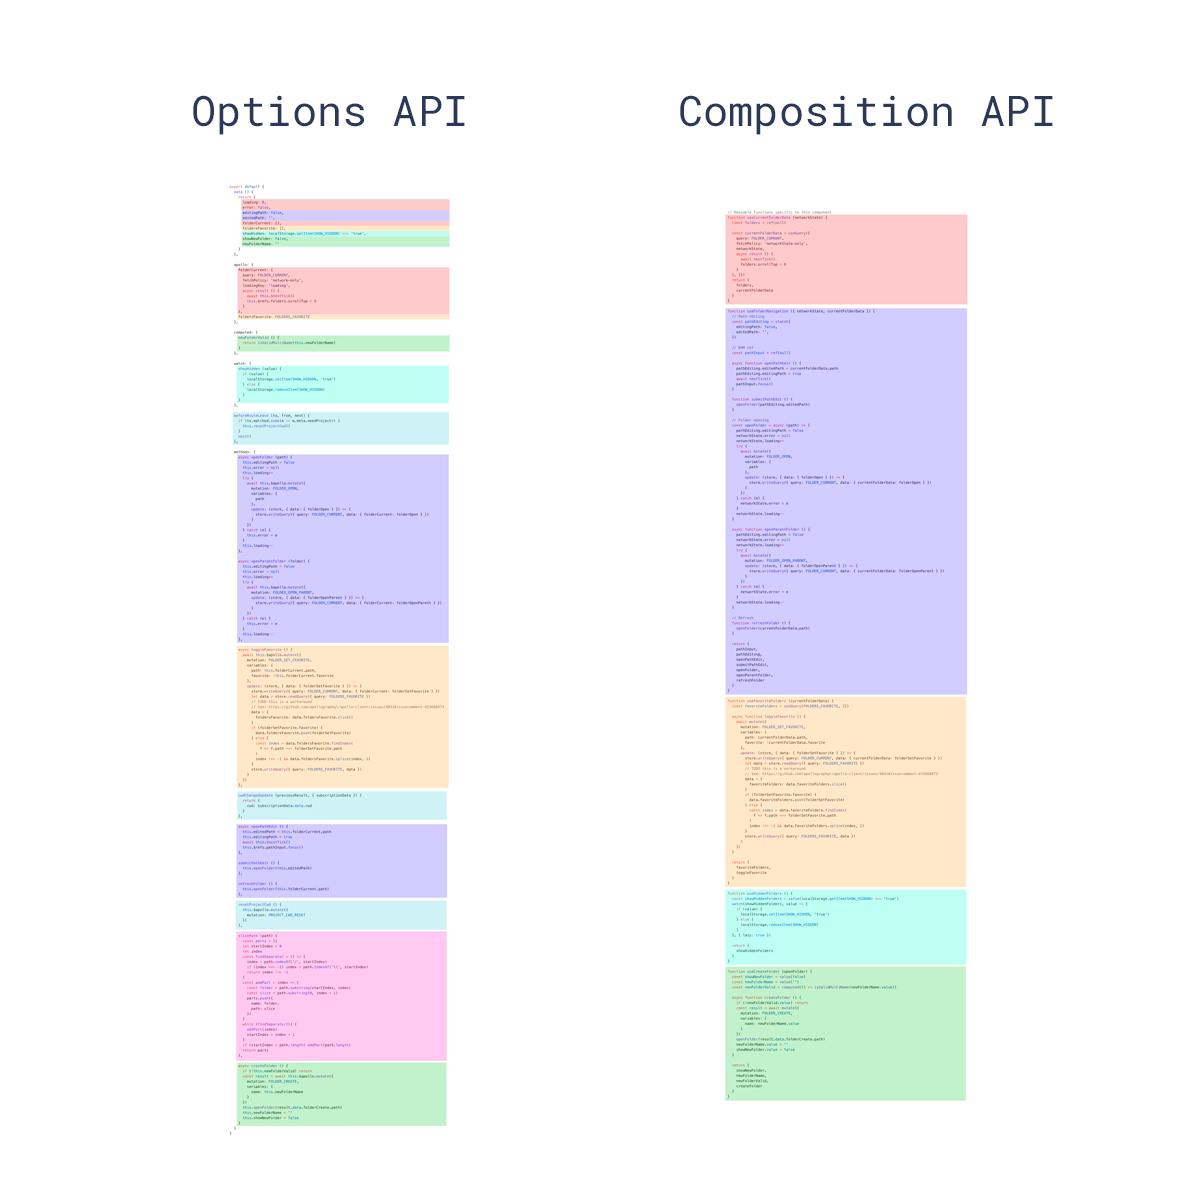
\includegraphics{./img/62783026-810e6180-ba89-11e9-8774-e7771c8095d6.png} 
\end{center}
     

\columnratio{0.55}
\begin{paracol}{2} 
 
\end{paracol}



\columnratio{0.55}
\begin{paracol}{2} 

\end{paracol}



\columnratio{0.55}
\begin{paracol}{2} 

\end{paracol}


\columnratio{0.55}
\begin{paracol}{2} 

\end{paracol}



\columnratio{0.55}
\begin{paracol}{2} 

\end{paracol}



\columnratio{0.55}
\begin{paracol}{2} 

\end{paracol}


\columnratio{0.55}
\begin{paracol}{2} 

\end{paracol}



\columnratio{0.55}
\begin{paracol}{2} 

\end{paracol}



\columnratio{0.55}
\begin{paracol}{2} 

\end{paracol}



\columnratio{0.55}
\begin{paracol}{2} 

\end{paracol}



\columnratio{0.55}
\begin{paracol}{2} 

\end{paracol}



\columnratio{0.55}
\begin{paracol}{2} 

\end{paracol}


\columnratio{0.55}
\begin{paracol}{2} 

\end{paracol}



\columnratio{0.55}
\begin{paracol}{2} 

\end{paracol}



\columnratio{0.55}
\begin{paracol}{2} 

\end{paracol}


\columnratio{0.55}
\begin{paracol}{2} 

\end{paracol}



\columnratio{0.55}
\begin{paracol}{2} 

\end{paracol}